\newpage
\section{Requisiti di sistema}
Il progetto Havana si presenta come una coppia di plugin per Kibana. Per questo motivo è necessario predisporre di Kibana correttamente installata e configurata con \gl{Elasticsearch}.
\\ Si garantisce una corretta visualizzazione e interazione con i plugin con Kibana v.6.
\subsection{Browser Supportati}

Di seguito viene fornito un breve elenco delle versioni minime dei browser sui quali il funzionamento dei nostri plugin è garantito:
\begin{itemize}
	
	\item \gl{Google Chrome} v.55
	\item \gl{Mozilla Firefox} v.50
	\item \gl{Safari} v.10
	\item \gl{Internet Explorer} v.11
	
\end{itemize}

Per un corretto funzionamento dei plugin è necessario che sia abilitato \gl{JavaScript}.

\section{Installazione del plugin}
Utilizzare il seguente comando per installare i plugin posizionati in un determinato \gl{URL}:
\begin{lstlisting}
 $ bin / kibana-plugin install < URL pacchetto>
\end{lstlisting}

Per l'installazione dei plugin su una \gl{directory} a scelta utilizzare l'opzione \texttt{-d} o \texttt{--plugin-dir} e dopo il comando \texttt{install} specificare una directory per i plugin, come nell'esempio seguente:
\begin{lstlisting}
 $ bin / kibana-plugin install file: ///some/local/path/my-plugin.zip -d path / to / directory 
\end{lstlisting}

Una volta completata l'installazione è possibile navigare tra tutti i plugin installati nella lista presente nel menù a sinistra di Kibana.

\newpage
\section{Mappa Topologica}
\label{sec:mtopologica}
\subsection{Interfaccia}

\begin{figure}[H]
	\centering 
	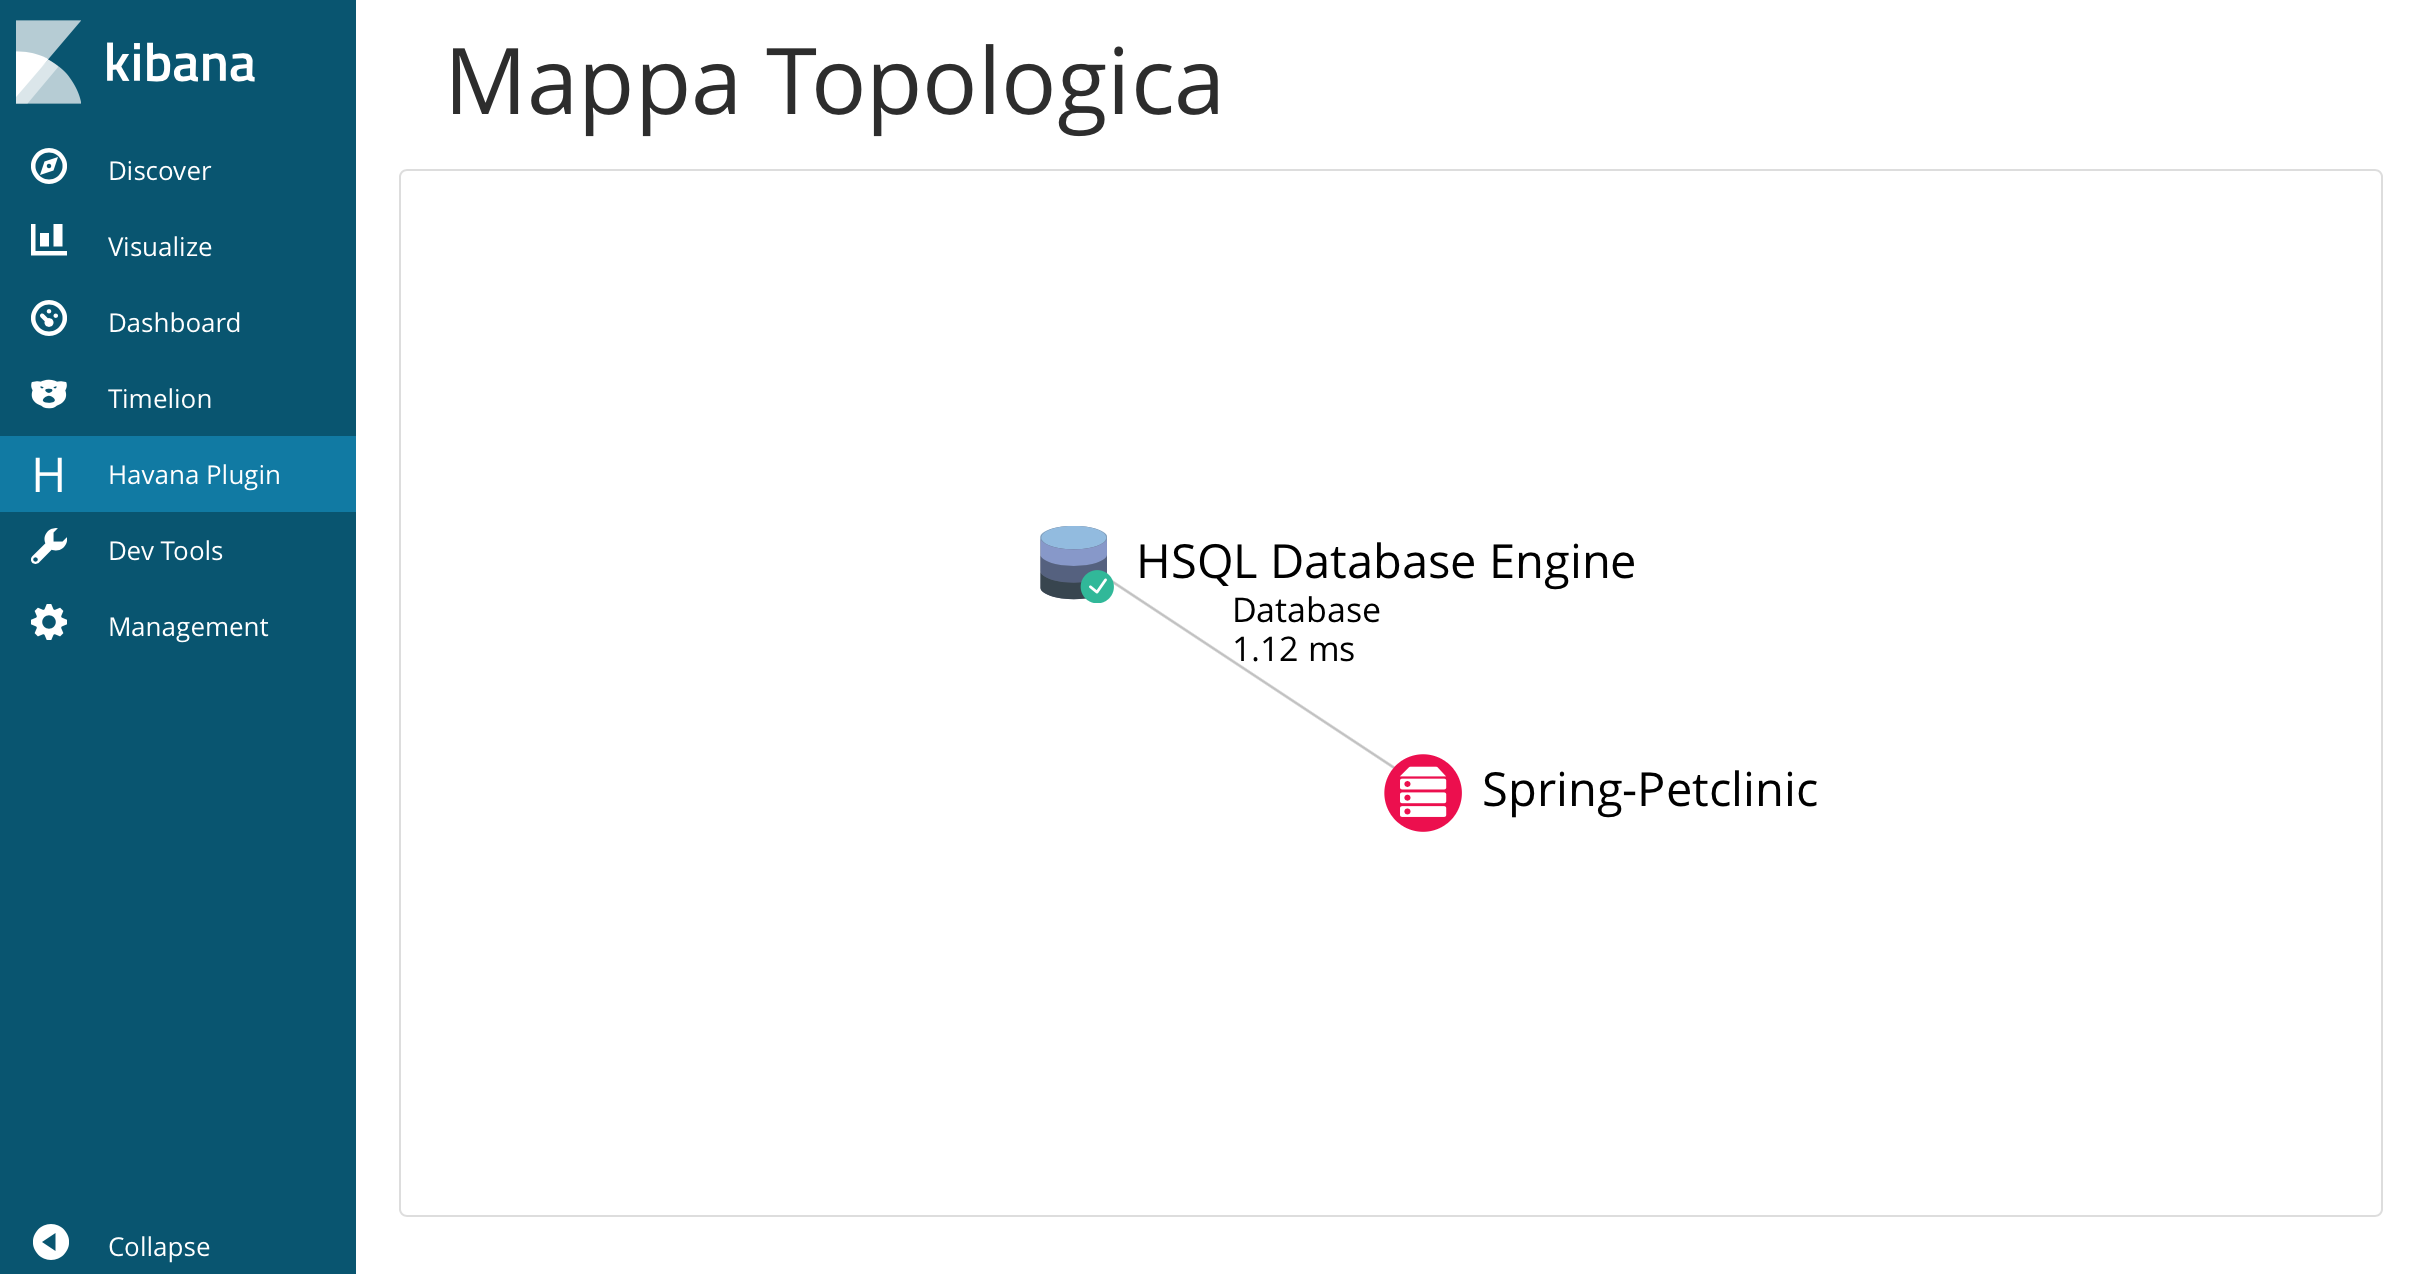
\includegraphics[width=1\textwidth]{Images/mappa}
	\caption{Visualizzazione del plugin Mappa Topologica}
\end{figure}

Questo plugin si presenta come una mappa nella quale vengono visualizzati i nodi \gl{hardware} di cui è composto il sistema dell'applicazione monitorata. 
I nodi vengono disegnati graficamente in maniera diversa a seconda della tipologia di componente che rappresentano ed ognuno viene affiancato dal nominativo. 
\\ I componenti che vengono visualizzati possono essere:
\begin{itemize}
	\item \emph{\gl{server}}, rappresentati attraverso un'icona circolare di colore rosso;
	\item \emph{\gl{database}}, rappresentati da un cilindro di colore blu e nero;
\end{itemize}
\begin{figure}[H]
	\centering 
	
\includegraphics[width=0.08\textwidth]{Images/server.png}
	\caption{Icona utilizzata per rappresentare i server}
	\label{server} 
\end{figure}
\begin{figure}[H]
	\centering 
	
\includegraphics[width=0.08\textwidth]{Images/database.png}
	\caption{Icona utilizzata per rappresentare i database}
	\label{database} 
\end{figure}

I componenti che interagiscono tra di loro sono collegati attraverso un arco che specifica  particolari informazioni:
\begin{itemize}
	\item etichetta con la tipologia dell'interazione;
	\item tempo medio di risposta.
\end{itemize}

\begin{figure}[H]
	\centering 
	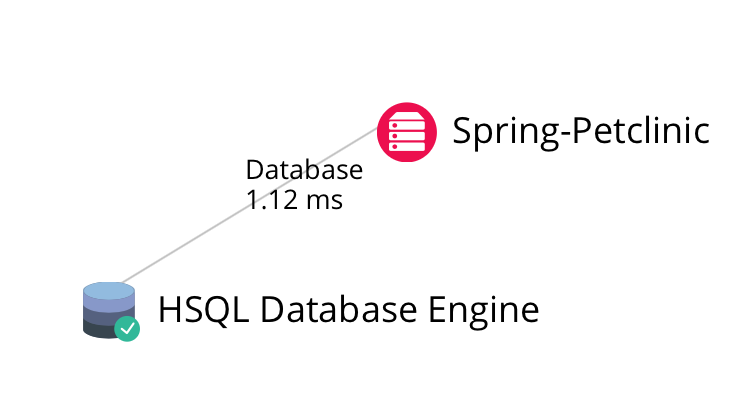
\includegraphics[width=0.5\textwidth]{Images/componenti}
	\caption{Esempio interazione tra due componenti}
\end{figure}

\subsection{Funzionalità}
    \subsubsection {Drag and Drop} 
Questa funzionalità permette di spostare i nodi della mappa nella posizione desiderata purchè sia all'interno dell'area del plugin il cui perimetro è evidenziato da un rettangolo di colore grigio.
Per spostare un nodo è necessario: 
\begin{enumerate}
	
	\item Portare il cursore del mouse sopra al nodo che si intende muovere;
	\item Cliccare e tenere premuto sul nodo;
	\item Spostare il nodo nella posizione desiderata.
	
\end{enumerate}

\subsubsection{Zoom}
Questà funzionalità permette all'utente di effettuare le operazioni di ingrandimento e rimpicciolimento delle dimensioni di visualizzazione della mappa. In particolare, è possibile ingrandire una specifica area della mappa.
Per effettuare questa operazione è necessario:

\begin{enumerate}
	
	\item Portare il cursore del mouse nel punto della mappa in cui si vuole effettuare l'operazione di zoom;
	\item Muovere la rotellina del mouse in avanti se si intende ingrandire, all'indietro se si intede rimpicciolire. Nel caso non si disponga della rotellina sul mouse, utilizzare le funzionalità presenti nella tastiera per effettuare lo zoom.
	
\end{enumerate}

\subsubsection{Tempo di risposta}
Questa funzionalità permette di visualizzare il tempo medio di risposta impiegato per effettuare richieste tra due nodi del sistema.
E' possibile visualizzarlo in corrispondenza della linea che collega due componenti.
Se il numero è colorato in rosso, significa che il tempo medio di risposta è superiore rispetto ad una soglia standard definita.




\section{Stack Trace}
\label{sec:strace}
\subsection{Interfaccia}
\begin{figure}[H]
	\centering 
	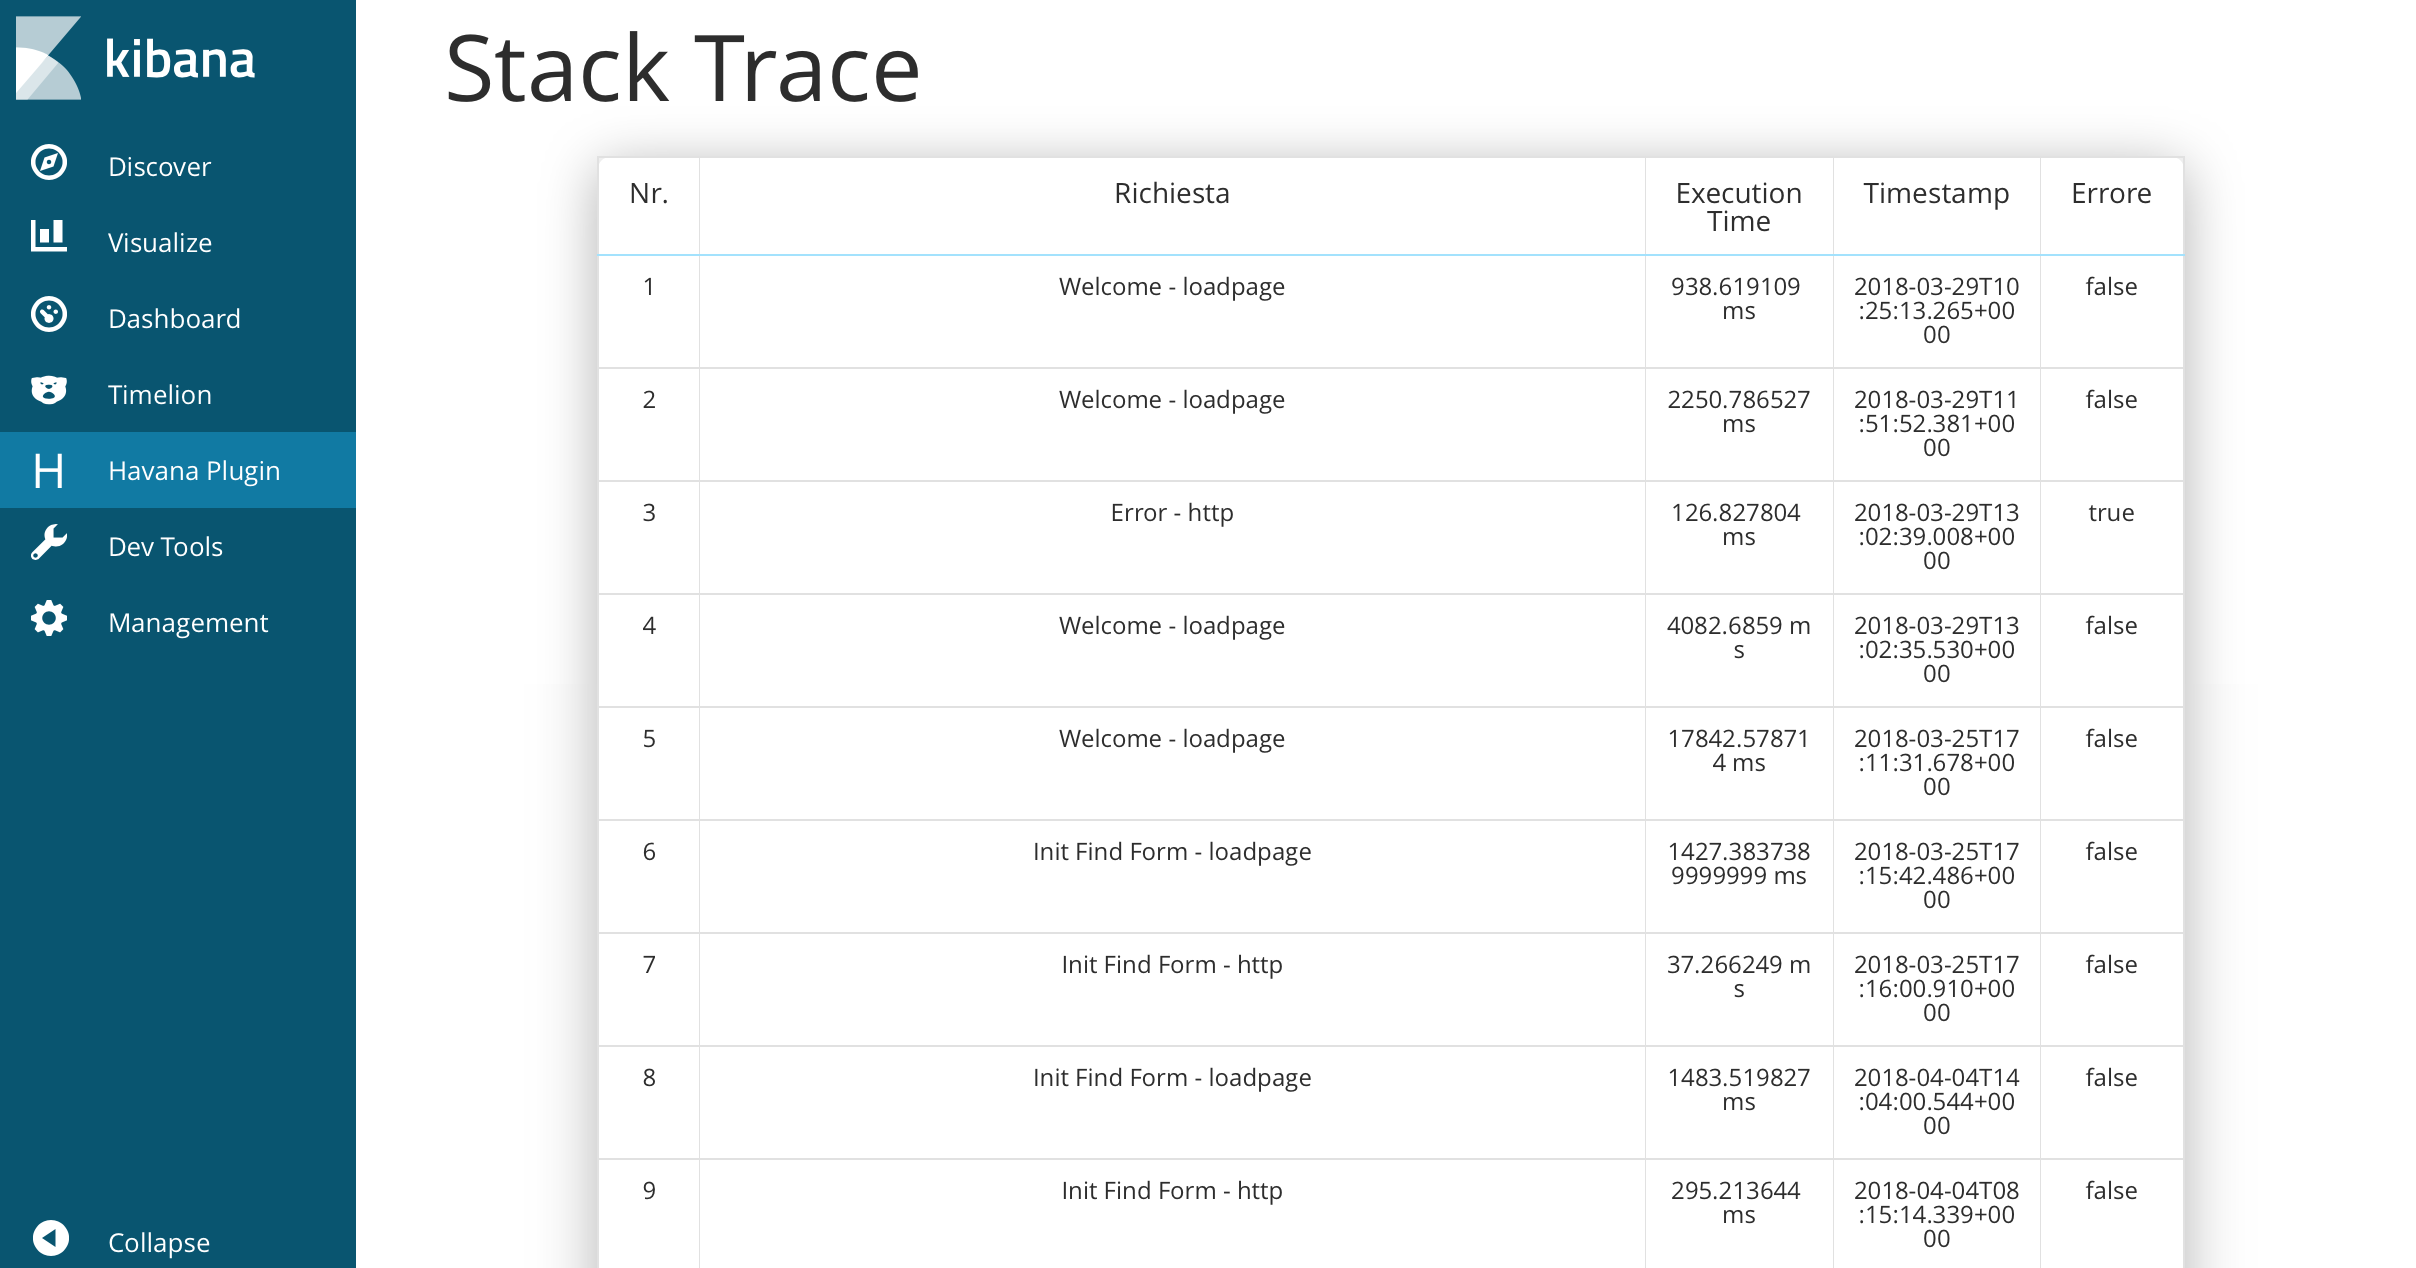
\includegraphics[width=1\textwidth]{Images/stack}
	\caption{Visualizzazione del plugin Stack Trace}
\end{figure}
Questo plugin rappresenta la lista di tutte le richieste effettuate dagli utenti al sistema dell'applicazione monitorata. Le richieste sono rappresentate in ordine cronologico decrescente e in più, per ogni richiesta, si possono visualizzare diverse informazioni.\\ Nello specifico:
   
    \begin{itemize}
    	
    	\item \textbf{Numero della richiesta:} numero progressivo associato alla richiesta;
    	\item \textbf{Richiesta:} nome della richiesta e tipologia;
    	\item \textbf{Execution Time:} tempo totale di esecuzione della richiesta;
    	\item \textbf{Timestamp:} indica l'istante temporale in cui è stata effettuata la richiesta;
    	\item \textbf{Errore:} indica se durante l'esecuzione della richiesta si è presentato qualche errore.
    	
    	\end{itemize}

\subsection{Funzionalità}
\subsubsection {Dettaglio richiesta}
Questa funzionalità permette di raggiungere un maggiore grado di dettaglio rispetto alle informazioni inizialmente rappresentate sulla tabella nella riga corrispondente alla richiesta di nostro interesse.
Per visualizzare maggiori informazioni riguardo una richiesta, l'utente deve cliccare sulla riga corrispondente.
\\Nell'estensione che appare è possibile, mediante il pulsante "switch", navigare nel \gl{Call Tree} o nella \gl{Query List} a seconda delle necessità.

\paragraph {Call Tree} \Spazio
\begin{figure}[H]
	\centering 
	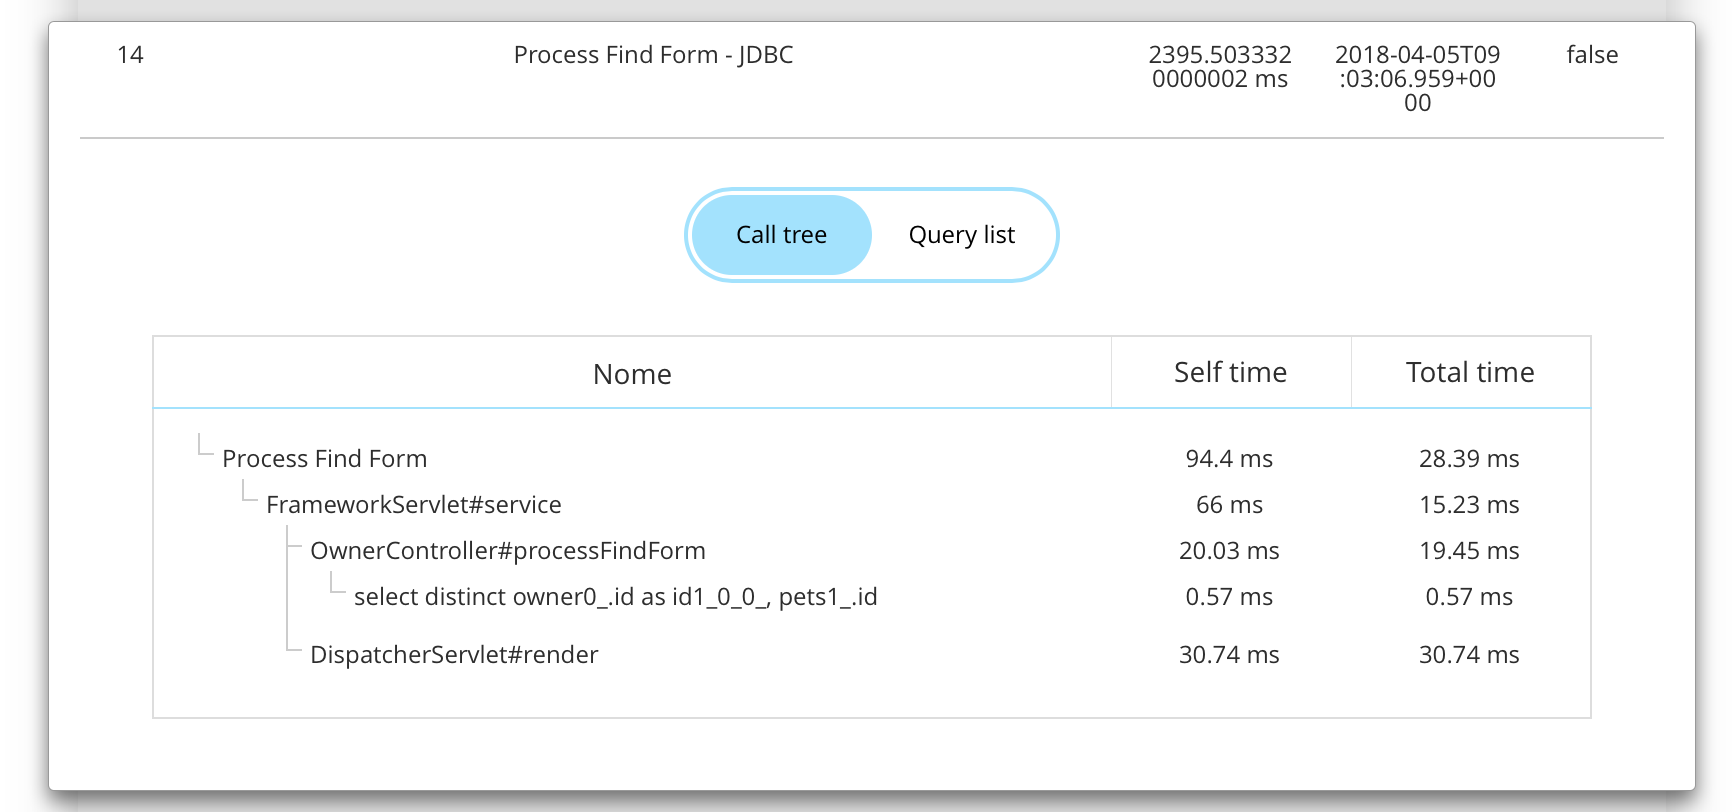
\includegraphics[width=1\textwidth]{Images/calltree}
	\caption{Visualizzazione del call tree di una richiesta}
\end{figure}
Il call tree rappresenta tutte le funzioni chiamate dal sistema per effettuare la richiesta dell'utente al sistema.
Ogni funzione è stata raffigurata in maniera indentata rispetto al padre così da riuscire a comprendere facilmente la gerarchia di annidamento.\\
E' possibile inoltre espandere/restringere ogni gerarchia di funzioni cliccando su di essa. In questo modo, tutta la gerarchia annidata verrà visualizzata/nascosta.

In corrispondenza di ogni funzione è possibile visualizzare il tempo di \emph{Self execution time} e il \emph{Total execution time}
\\

\paragraph {Query List} \Spazio
\begin{figure}[H]
	\centering 
	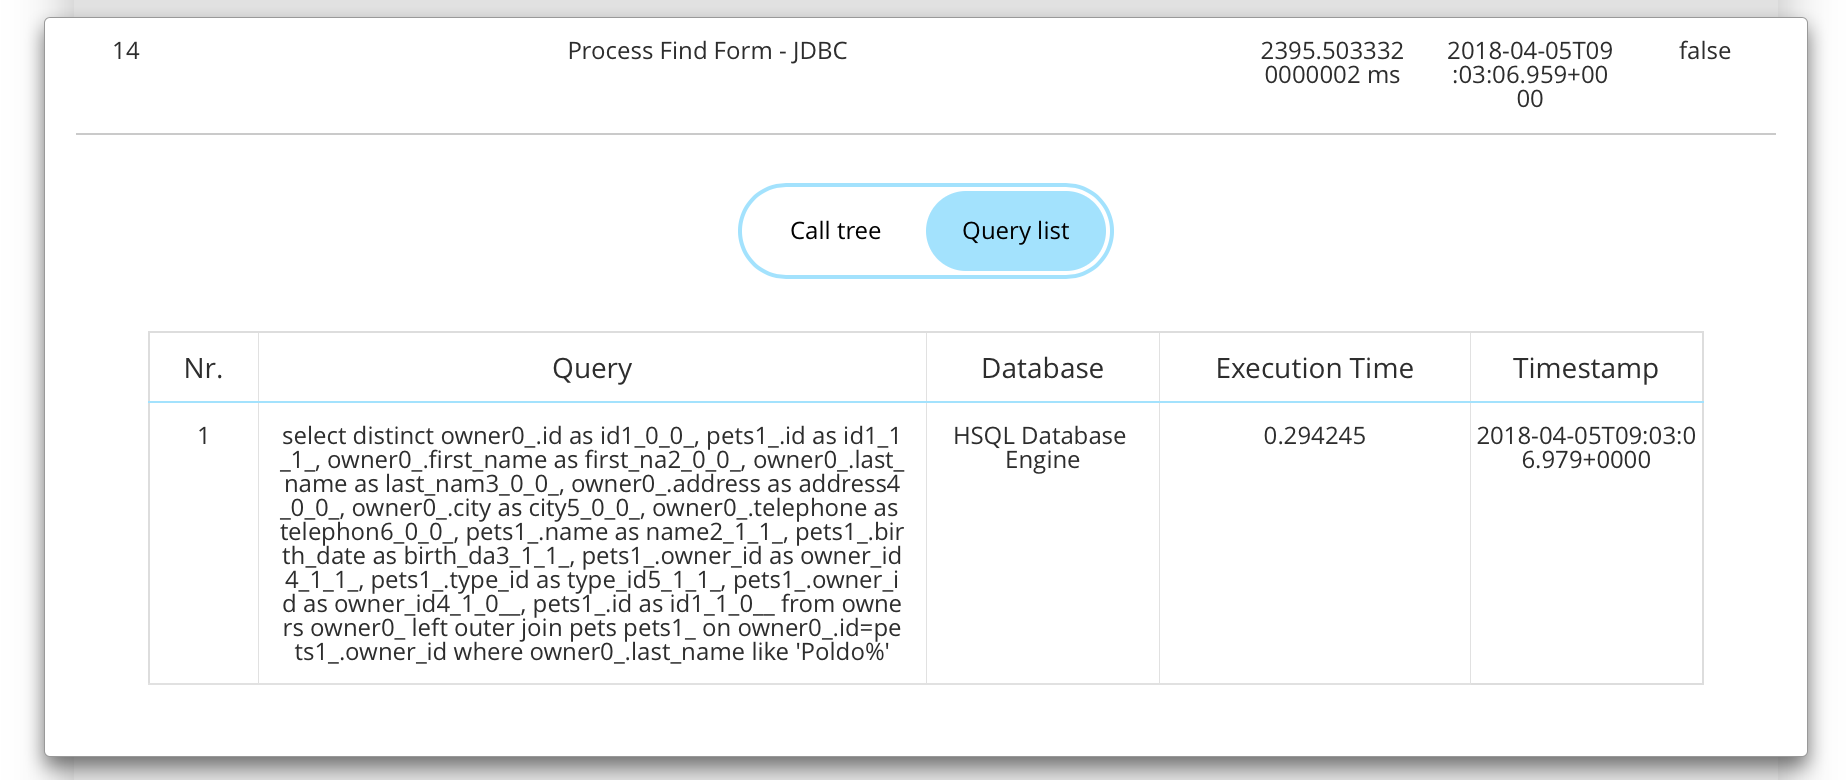
\includegraphics[width=1\textwidth]{Images/querylist}
	\caption{Visualizzazione delle query associate ad una richiesta}
\end{figure}
Rappresenta tutte le query effettuate nel database dal sistema per fornire una risposta alla richiesta dell'utente.
    \begin{itemize}
	
	\item \textbf{Numero della query:} numero progressivo associato alla query;
	\item \textbf{Query:} testo della query effettuata;
	\item \textbf{Database:} nome del database nel quale è stata effetuata la query;
	\item \textbf{Execution Time:} tempo impiegato dalla query per fornire un risultato;
	\item \textbf{Timestamp:} indica l'instante temporale in cui è stata effettuata la query.
	
\end{itemize}



\newpage
\appendix
\section{Glossario}
\lettera{C}

\parola{Call tree}{Albero delle chiamate, rappresenta l'insieme delle chiamate a funzioni o funzionalità del sistema eseguite da un programma.}

\parola{Cluster}{Insieme di computer connessi tra loro tramite una rete telematica. Lo scopo di un cluster è quello di distribuire una elaborazione molto complessa tra i vari computer.}


\lettera{D}

\parola{Database}{Archivio di dati strutturato in modo da razionalizzare la gestione e l'aggiornamento delle informazioni e da permettere lo svolgimento di ricerche complesse.}

\parola{Directory}{Entità del file system che elenca altre entità, tipicamente file e altre directory, e che permette di organizzarle in una struttura ad albero.}

\lettera{E}

\parola{Elastic Search}{Motore di ricerca open-source. Dispone di API molto estensive ed elaborate. Può effettuare ricerche in maniera molto perfomante.}

\lettera{G}
\parola{Google Chrome}{Google Chrome è un browser web sviluppato da Google, basato sul motore di rendering Blink.}

\lettera{H}
\parola {Hardware}{Insieme delle componenti fisiche, non modificabili, di un sistema di elaborazione dati.}

\lettera{I}
\parola{Internet Explorer}{Browser web grafico proprietario sviluppato da Microsoft e incluso in Microsoft Windows a partire dal 1995.}

\lettera{J}

\parola{JavaScript}{Linguaggio di scripting utilizzato principalmente per applicazioni web.}

\lettera{K}

\parola{Kibana}{Framework open source per la visualizzazione dei dati salvati su Elasticsearch.}

\lettera{M}

\parola{Mappa topologica}{Visualizzazione sotto forma di grafo dei componenti di un'applicazione in cui i componenti come server e database sono i nodi e le interazioni fra essi, ovvero le richieste fatte da un componente ad un altro (come richieste HTTP o queries), sono gli archi.}

\parola{Mozilla Firefox}{Web browser libero e multipiattaforma, mantenuto da Mozilla Foundation.}

\lettera{P}
\parola{Plugin}{Programma non autonomo che interagisce con un altro programma per ampliare o estendere le funzionalità originarie.}  

\parola{Prodotto}{Indica il risultato di un'attività, sia esso un documento, del codice sorgente o un qualsiasi risultato verificabile che possa essere offerto per soddisfare un bisogno o un’esigenza.}  

\parola{Progetto}{Insieme di attività e compiti che prevedono il raggiungimento di determinati obiettivi con specifiche fissate. Sono definite date di inizio e fine durante la quale si può predisporre di limitate risorse che vengono consumate nello svolgersi delle attività. }  

\lettera{S}

\parola{Safari}{Web browser multipiattaforma, sviluppato e mantenuto da Apple.}

\parola{Stack Trace}{Lista di un insieme di traces prese in esame.}

\lettera{T}

\parola{Trace}{Struttura dati che rappresenta una singola richiesta effettuata fra due componenti di una applicazione monitorata oppure fra un utente esterno e un componente dell'applicazione. Viene solitamente memorizzata in un database per successiva analisi.}

\lettera{U}

\parola{URL}{\emph{Uniforme Resource Locator}, indirizzo simoboli per riferirsi ad una risorsa in rete.}

